\section{Wavelet Thresholding Algorithm}\label{sec:wavelet-thresholding-algorithm}

\jsm{[MENTION THE ALGORITHM FOR JOINT WAVELET COMPRESSION IS DETAILED IN THE MORRIS ET AL. 2008 BIOMETRICS PAPER]}We use the Discrete Wavelet Transform (DWT) algorithm implementation in the \texttt{dwt()} function from the \pkg{wavselim} \proglang{R} package \parencite{whitcher_waveslim_2024}.
Our thresholding approach is described below, and demonstrated on the \texttt{DTI} dataset from the \pkg{refund} \proglang{R} package \parencite{goldsmith_refund_2020}.
As our main focus is on the technical setps of the wavelet decomposition, we describe the selection of the coefficients on the same sample of data that we want to reconstruct. However, in practice, Steps 3 and 4 would only be performed on the training data and then test/ validation data used to assess generalisation error using a chosen truncation.

\begin{steps}
  \item \underline{\textbf{Pad the Data to Dyadic Length}}: The DWT can only be applied to vectors of dyadic length, i.e., a power of $2$. In most cases, the we work with the $N \times T$ data matrix $\mathbf{X}$ where $T$ is not a power of $2$ (i.e., $\log_2(T)$ is not an integer). If this is the case, we define $\log_2(T_{pad})$ as the smallest integer greater than $\log_2(T)$. We then add $\lceil (T_{pad} - T)/2 \rceil$ columns of $0$'s to the left and $\lfloor (T_{pad} - T)/2 \rfloor$ columns of $0$'s to the right side of $\mathbf{X}$, so that the resulting matrix $\mathbf{X}_{pad}$ has dimensions $N \times T_{pad}$ (Figure \ref{fig:DTI-padded}).
  \begin{figure}[H]
      \centering
      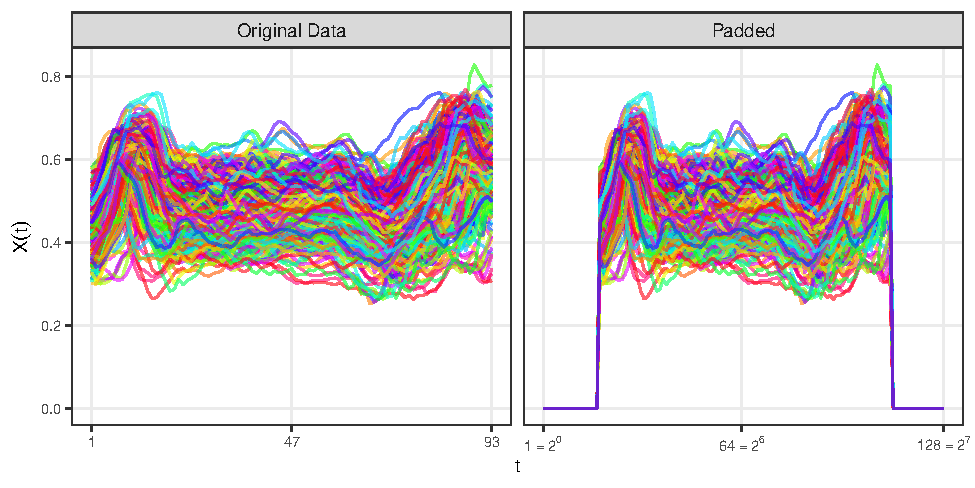
\includegraphics[width=0.75\linewidth]{figures/DTI-padded.pdf}
      \caption{Padding the \texttt{DTI} data to transform it from length $T = 93$ to $T_{pad} = 128 = 2^7$.}
      \label{fig:DTI-padded}
  \end{figure}
  \item \underline{\textbf{Apply the DWT to Each Row}}: We then apply the DWT to each row of $\mathbf{X}_{pad}$, which transforms each vector from $T_{pad}$ measurements of a time series (or signal) to $T_{pad}$ wavelet coefficients.
  By default, the \texttt{waveslim::dwt()} function employs ``the Daubechies orthonormal compactly supported wavelet of length L=8 \parencite{daubechies_ten_1992}, least asymmetric family" as the wavelet filter, with periodic assumptions for the signal beyond the boundaries \parencite[][p.7]{whitcher_waveslim_2024}.
  We add store the wavelet coefficients for each row in the rows of the $N \times T_{pad}$ matrix $\mathbf{X}^*$.
  When we have expanded the original signal by padding in Step 1, we can expect a number of the $T_{pad}$ wavelet coefficients to be $0$, however this number is likely to be less than $T_{pad} - T$.
  \item \underline{\textbf{Compute the Relative Energy Matrix}}: For each row of $\mathbf{X}^*$, we have the vector of wavelet coefficients $\mathbf{X}^*_{i\cdot} = (X^*_{i1}, \dots,X^*_{iT_{pad}})^\top$. We denote the \emph{Total Energy} for the $i$th observation as the sum of its squared wavelet coefficients
  $$\text{Total Energy}_i = \sum_{k=1}^{T_{pad}}X^{*2}_{ik}.$$ Next, we define the \emph{Cumulative Relative Energy} for the $i$th observation and wavelet coefficient $k$ as 
  $$
  \text{Relative Energy}_{ik} = \frac{\sum_{\{k: \lvert X^*_{ik'}\rvert  \geq \lvert X^*_{ik}\rvert \}}X^{*2}_{ik}}{\text{Total Energy}_i}.
  $$
  This quantity represents the proportion of the total energy that is explained by the $k$th wavelet coefficient and all coefficients greater in absolute value than it. Hence, smaller values indicate this coefficient is important and values closer to $1$ indicate less importance (i.e., a value of $1$ indicates that all of the energy has been explained before this coefficient).
  Normalising by the total energy is important because we summarise this quantity across all $i$ as a measure of importance in the next step, and the normalisation ensures that it the importance is not obscured by the total energy of an individual signal. We let $\textbf{En}^*$ represent the total energy matrix which contains $\text{Relative Energy}_{ik}$ in its $i$th row and $k$th column.
  \item \underline{\textbf{Compute the Relative Energy Scree}}: To summarise the overall importance of each of the wavelet coefficients we average each column of the matrix $\textbf{En}^*$. We obtain the $T_{pad}$-dimensional \emph{Scree} vector, that has the $k$th entry
  $$
  \text{Scree}_k = \frac{1}{N} \sum_{i=1}^N \text{Relative Energy}_{ik}.
  $$
  As with the individual relative energy matrix, coefficients with a lower average value are of greater importance while larger average values (closer to $1$) indicate less importance.
  \item \underline{\textbf{Hard Thresholding Based on the Relative Energy Scree}}: For a given $K < T_{pad}$, we threshold the wavelet coefficient matrix $\mathbf{X}^*$ based on the relative energy scree. That is, we retain the $K$ columns of $\mathbf{X}^*$ that have the smallest values of $\text{Scree}_k$ and set the remaining columns to $0$. We denote the thresholded version of $\mathbf{X}^*$ by $\widehat{\mathbf{X}}^{*(K)}$.
  \item \underline{\textbf{Apply IDWT to Each Row of the Thresholded Coefficient Matrix}}: To transform back to the data space, we apply the inverse DWT (IDWT) to each row of $\widehat{\mathbf{X}}^{*(K)}$. This will give use the reconstructed matrix $N\timesT_{\pad}$
  $$
  \widehat{\mathbf{X}}^{(K)}_{pad} = \text{IDWT}(\widehat{\mathbf{X}}^{*(K)}).
  $$
  To obtain a representation of the original signal length we simply discard the first $\lceil (T_{pad} - T)/2 \rceil$ columns and the last $\lfloor (T_{pad} - T)/2 \rfloor$ columns to give the matrix $\widehat{\mathbf{X}}^{(K)}$. Figure \ref{fig:DTI-recon} displays the reconstruction of the \texttt{DTI} data using differing values of $K$, alongside the original data.
  \begin{figure}[H]
      \centering
      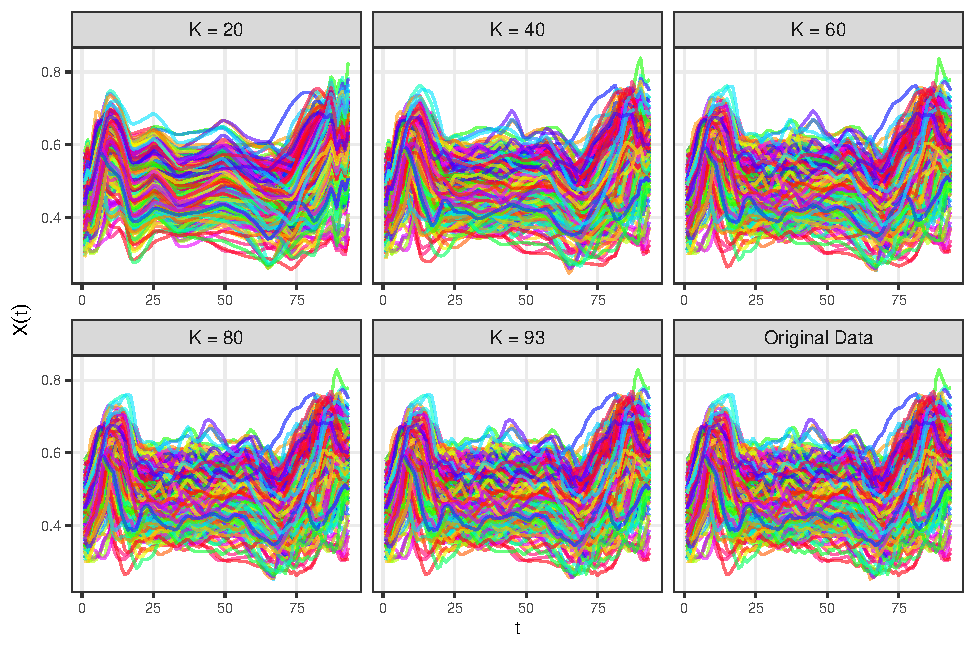
\includegraphics[width=0.8\linewidth]{figures/DTI-recon.pdf}
      \caption{Thresholded wavelet representations of the \texttt{DTI} data with differing values of $K$, alongside the original data (bottom right).}
      \label{fig:DTI-recon}
  \end{figure}
\end{steps}
